\section{Proposed Method}

In this section a detailed description of the proposed algorithm is given to the lecturer: 
some implemented procedures will be explained through pseudocode. 
The algorithm works in successive stages as described in the following:

\begin{itemize}
    \item Kernel loading
    \item Image reading
    \item Output Image creation
    \item Image selection, enlargement and filling
    \item Image enhancement
\end{itemize}

The algorithm is divided into two parts: the first one focuses on the CPU, which is responsible for the reading of the image
and the kernel loading; the second one is the GPU part, which is responsible for the image cut out, enlargement, filling, and enhancement.
The inputs required by the application are based on the commands given by the user through the command line, and they are the following:
\begin{itemize}
    \item The path of the image to be zoomed;
    \item The -$c$ (--$custom$) flag, which refers to a custom kernel, followed by the file path of the kernel;
    \item The -$g$ (--$gauss$) flag, which refers to a Gaussian kernel, followed by the length of the kernel and the $\Sigma$ value, mutually exclusive with the previous;
    \item An optional $v$ character, appended to the mode, which enables the verbose mode;
    \item An optional $f$ character, which forces the use of global memory instead of the shared;
    \item The coordinates of the center of the cut-out area, in the form of $x,y$;
    \item The width and the height of the cut-out area;
    \item The zoom level of the image must be an integer bigger than 0, it represents the multiplier of the cut-out area dimension;
\end{itemize}

\begin{lstlisting}[language=bash]
    # Example of command line with gaussian kernel
    # cutout center (100,100), zoom 2, dimensions 50x50, kernel size 31, sigma 5
    upsCu -g ./img.ppm 100 100 50 50 2 31 5 
    # Example of command line with custom kernel
    # cutout center (100,100), zoom 2, dimensions 50x50, kernel file ./kernel.txt
    upsCu -c ./img.ppm 100 100 50 50 2 ./kernel.txt
    # Example of command line with global memory
    # cutout center (100,100), zoom 2, dimensions 50x50, kernel size 31, sigma 5
    upsCu -gf ./img.ppm 100 100 50 50 2 31 5 
    # Example of command line with verbose mode
    # cutout center (100,100), zoom 2, dimensions 50x50, kernel size 31, sigma 5
    upsCu -gv ./img.ppm 100 100 50 50 2 31 5
\end{lstlisting}

    \subsection{Kernel Loading}
    The algorithm can choose between custom kernels loaded from files, or Gaussian ones, which are generated on the fly,
    taking as input the length of the kernel and the standard deviation.
    
    %Gaussian kernel generation equation
    \begin{equation}
        \label{eq:gauss}
        G(x,y) = \frac{1}{2\pi\sigma^2}e^{-\frac{x^2+y^2}{2\sigma^2}}
    \end{equation}
    
    The kernel is generated by using the equation above, iterating over the matrix length, 
    and then normalizing it. The normalization is done by dividing each value of the matrix by the sum of all the values of the matrix.
    %Gaussian kernel generation pseudocode
    \noindent\small\begin{lstlisting}[language=C]
...
kernel[i][j]=exp(-((i - kernel_size / 2) * (i - kernel_size / 2)
    + (j - kernel_size / 2) * (j - kernel_size / 2)) / 
    (2 * sigma * sigma)) / (2 * M_PI * sigma * sigma);
...
kernel[i][j] /= sum;
...
/* Load into constant memory */
cudaMemcpyToSymbol(d_kernel, kernel, dimKernel * dimKernel * sizeof(float));
    \end{lstlisting}

    Once generation is done, the kernel is loaded into 
    GPU's constant memory, which allows the program to save time. This happens because constant memory is a special type of global memory 
    with a peculiar cache that doesn’t need to do as many coherency tests as the other caches. This is useful because every value of the mask is read at the same 
    time by every thread of the program, and it is not modified during the execution of the program.\\
    The \textit{GaussLength} parameter must be an odd value from 3 to 127 sides included and the \textit{GaussSigma} parameter must be a value from 0.5 onwards side included.
    The custom kernel must be a square matrix, and it has to be at maximum \textit{MAX\_KERNEL\_DIM} long, which is set to 127 elements.
    %mettere qui foto distribuzione gaussiana 

    \subsection{Image Cut-Out}
    The aim of this step is to select the part of the original image that has to be trimmed: 
    the dimensions of the cut area are passed through command line and the script subsequently calculates the dimension of the output image.\\ 
    The function carries out the logic explained down below:


    \noindent\begin{lstlisting}[language=C]
...
img_out[tid] = img[starting_byte+row_offset+column_offset]
...
    \end{lstlisting}

    \noindent Where $tid$ is the thread ID, $img\_out$ is the final image, $img$ is the original image, $starting\_byte$ is the starting byte of the cut area, 
    $row\_offset$ is the offset of the row of the pixel to be copied and $column\_offset$ is the offset of the column of the pixel to be copied.
    The implementation is basic, it is a simple copy of the pixels from the original image to the final one, done in parallel using CUDA threads.\\

    \subsection{Image Enlargement and Filling}
    This step is the one that enlarges the image and fills the holes that are created by the zooming process.
    The process begins by creating as many threads as the bytes in the final image, and each one of them computes 
    the value of the pixel to be copied from the original image.
    The holes are filled with the help of the pixel replication algorithm. 

    \small\noindent\begin{lstlisting}[language=C]
...
int stuffing = dimImgMid / dimImgIn * 3;
if (idx >= dimImgMid * dimImgMid * 3)
{
    return;
}
rowOffset = offset * dimImgOut * 3;
colOffset = offset * 3;
outputRowOffset = idx / 3 / dimImgMid * dimImgOut * 3;
outputColOffset = idx / 3 % dimImgMid * 3;
position = colOffset + rowOffset + outputRowOffset + outputColOffset + idx%3;
offsetScaledRow = idx / dimImgMid / stuffing * dimImgIn * 3;
offsetScaledCol = (idx / 3 % dimImgMid) / stuffing * 9;
scaled_img[position] = cutout[offsetScaledRow + offsetScaledCol + idx%3];
...
    \end{lstlisting}


    It replicates the neighboring pixels in order to increase them to enlarge the image, based on the zoom factor. It is the most basic technique to implement
    zooming, but it is the most efficient one since it does not require any computation.\\
    In the first version of the algorithm the canvas gets filled with the enlarged image and black borders around it,
    which will be used to perform the convolution with the filter, since it needs a larger image than the one that is actually returned as output.

    \noindent\begin{lstlisting}[language=C]
...
if ((row_i >= 0) && (row_i < inHeight) && (col_i >= 0) && (col_i < inWidth))
{
    in_img_shared[ty * blockDim.x + tx] = input[(row_i * inWidth + col_i) * 3 + color];
}
else
{
    in_img_shared[ty * blockDim.x + tx] = 0;
}
...
    \end{lstlisting}


    The final version of the algorithm instead gets directly the pixels needed and if the cut-out is not at the border, the program will use neighboring pixels
    to create a slightly bigger image for the convolution. If the cut-out is at the border, the nearest pixel will be used just for the border part.
    This final version produces an image which is really close to the original one.\\

    \begin{figure}
        \centering
        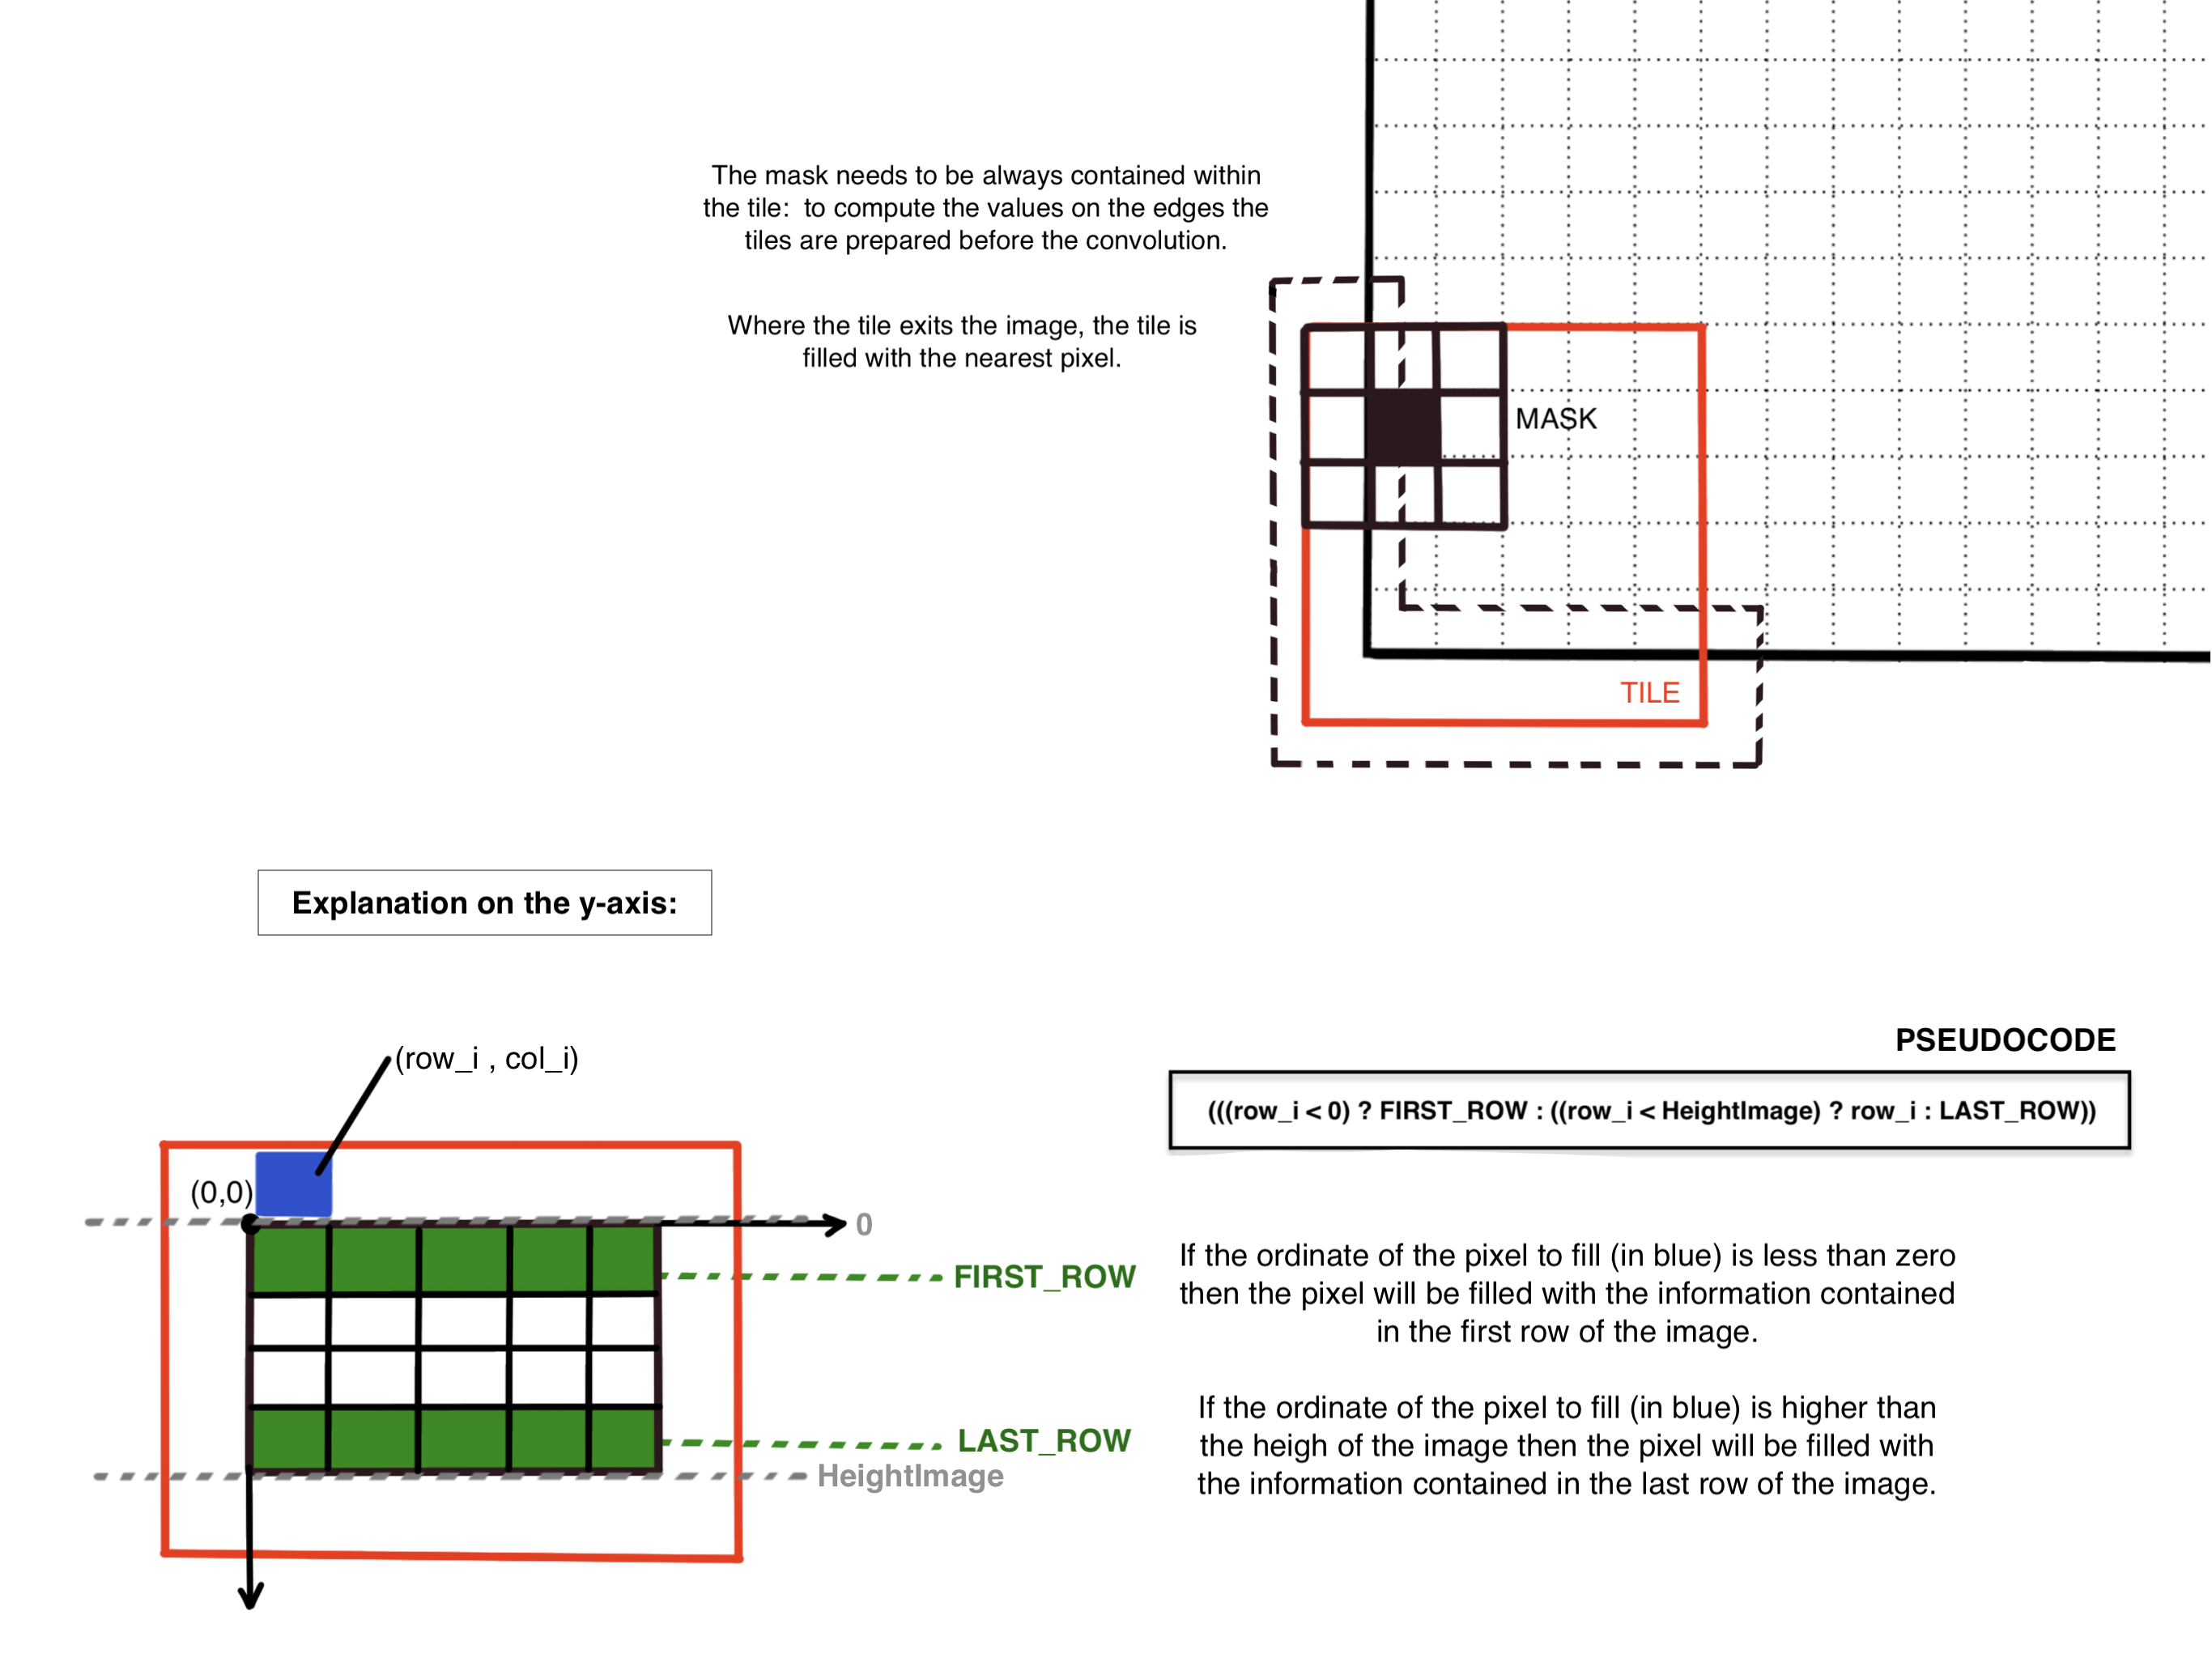
\includegraphics[width=0.75\textwidth]{img/EDGEscheme.png}
        \caption{Border pixel replication (same happens for columns)}
        \label{fig:borderrepl}
    \end{figure}


    \subsection{Image Enhancement}
    This step executes the convolution of the image with the kernel, in order to enhance the image and make it clearer.\\
    Many versions of the algorithm have been tested, starting from only using global memory, to using shared memory and tiling technique.\\
    The first version of the program, which uses only global memory, performs the operations slower than the other,
    but it is the most straightforward one used as workbench. The function remains available for the user, when needed. The second version of the algorithm, improves the performances of the algorithm, by exploiting the shared memory,
    which allows to have a faster access to the data. This happens because it is a cache located on chip, thus accessible by all threads of a block, 
    providing a mechanism for threads to cooperate, while diminishing the access to global memory stored in the DRAM.
    These main problems arise when using shared memory: the fact that it is limited in size, it is not possible to use it for all the data needed 
    and bank conflicts. The last issue is caused by the shared memory division into banks which can be accessed simultaneously by different threads
    only if they are accessing different registers. This means that if two threads are accessing the same bank, they will have to wait for the other one to finish,
    and this will cause a slowdown in the execution of the algorithm.
    The tiling technique is preferred because it uses the shared memory and the commodities and hacks that comes with it, avoiding conflicts.
    The image is divided into tiles, convolution is then performed on each of them and the result is the final image. This technique allows avoiding bank conflicts, because each tile is stored in a different
    bank, reducing memory traffic.
    
    \noindent The basic version of the algorithm uses a kernel created by the \textit{Gaussian\_Kernel\_Cpu} function stored in constant memory referenced by \textit{d\_kernel}. 
    It computes the convolution using one thread for each byte of the image by dividing it in blocks of the same size. 
    The convolution is performed per color channel, using blocks of pixels of the same dimension of the kernel, centered in the pixel to be processed.
    The result is achieved by multiplying the value of the pixel with the value of the corresponding element of the kernel, and then summing all the results.

    The final version, with shared memory and tiling, decides if the image is large enough to be tiled by computing the width of the tile:
    \noindent\begin{lstlisting}[language=C]
...
heightTile = widthTile = \sqrt{maxThreadsPerBlock} - (maskDim - 1);
setTiling(widthImgOut, heightImgOut, &widthTile, &heightTile);
...
    \end{lstlisting}
    
    \noindent If the product of \textit{heightTile} and \textit{widthTile} is bigger than one, the tiling technique is performed, otherwise the global memory version is used because the tiling technique would not be efficient
    due to the overhead of the tiling process.
    The shared memory has to be filled first with the color information of the image, then used to perform the convolution with the mask.
    All the initialized threads of the block participate in filling the memory but afterwards only some of them participate in calculating the convolution with the mask for that block.
    The number of threads set for each block corresponds to the number of bytes allocated for the shared memory: in the project it is set to $bigTileDimX*bigTileDimY$.

    \begin{figure}
        \centering
        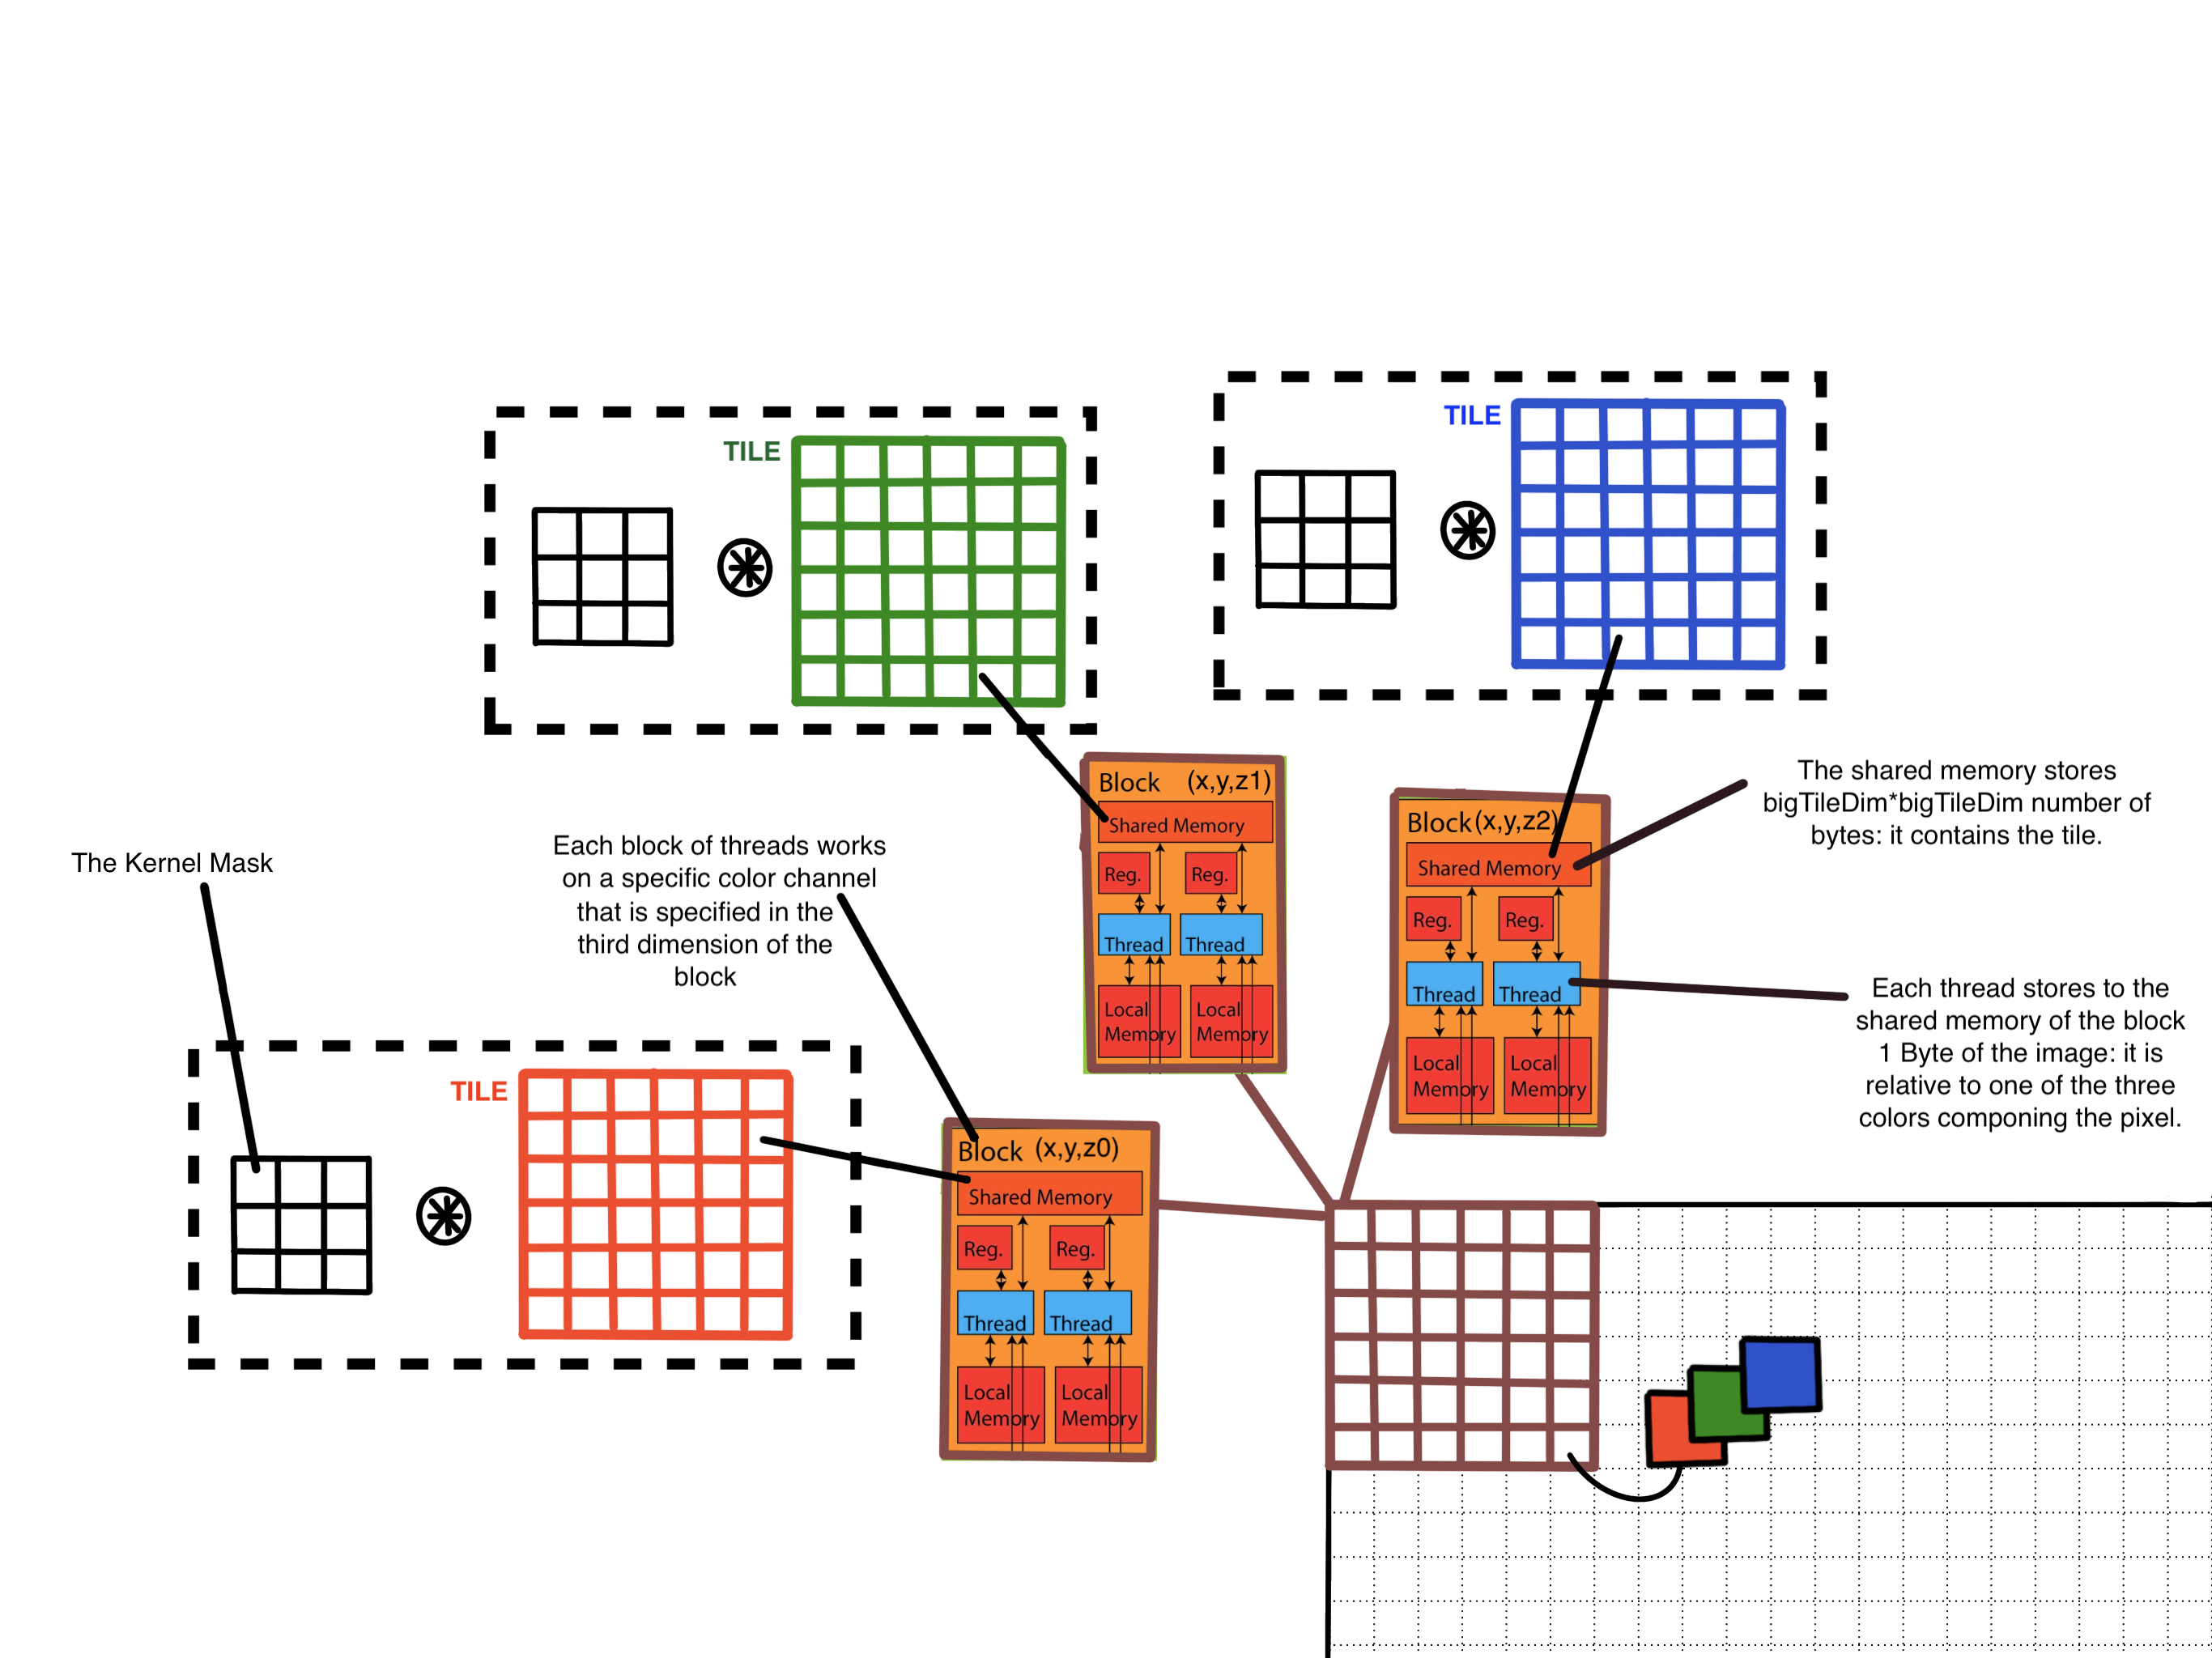
\includegraphics[width=0.7\textwidth]{img/scheme.png}
        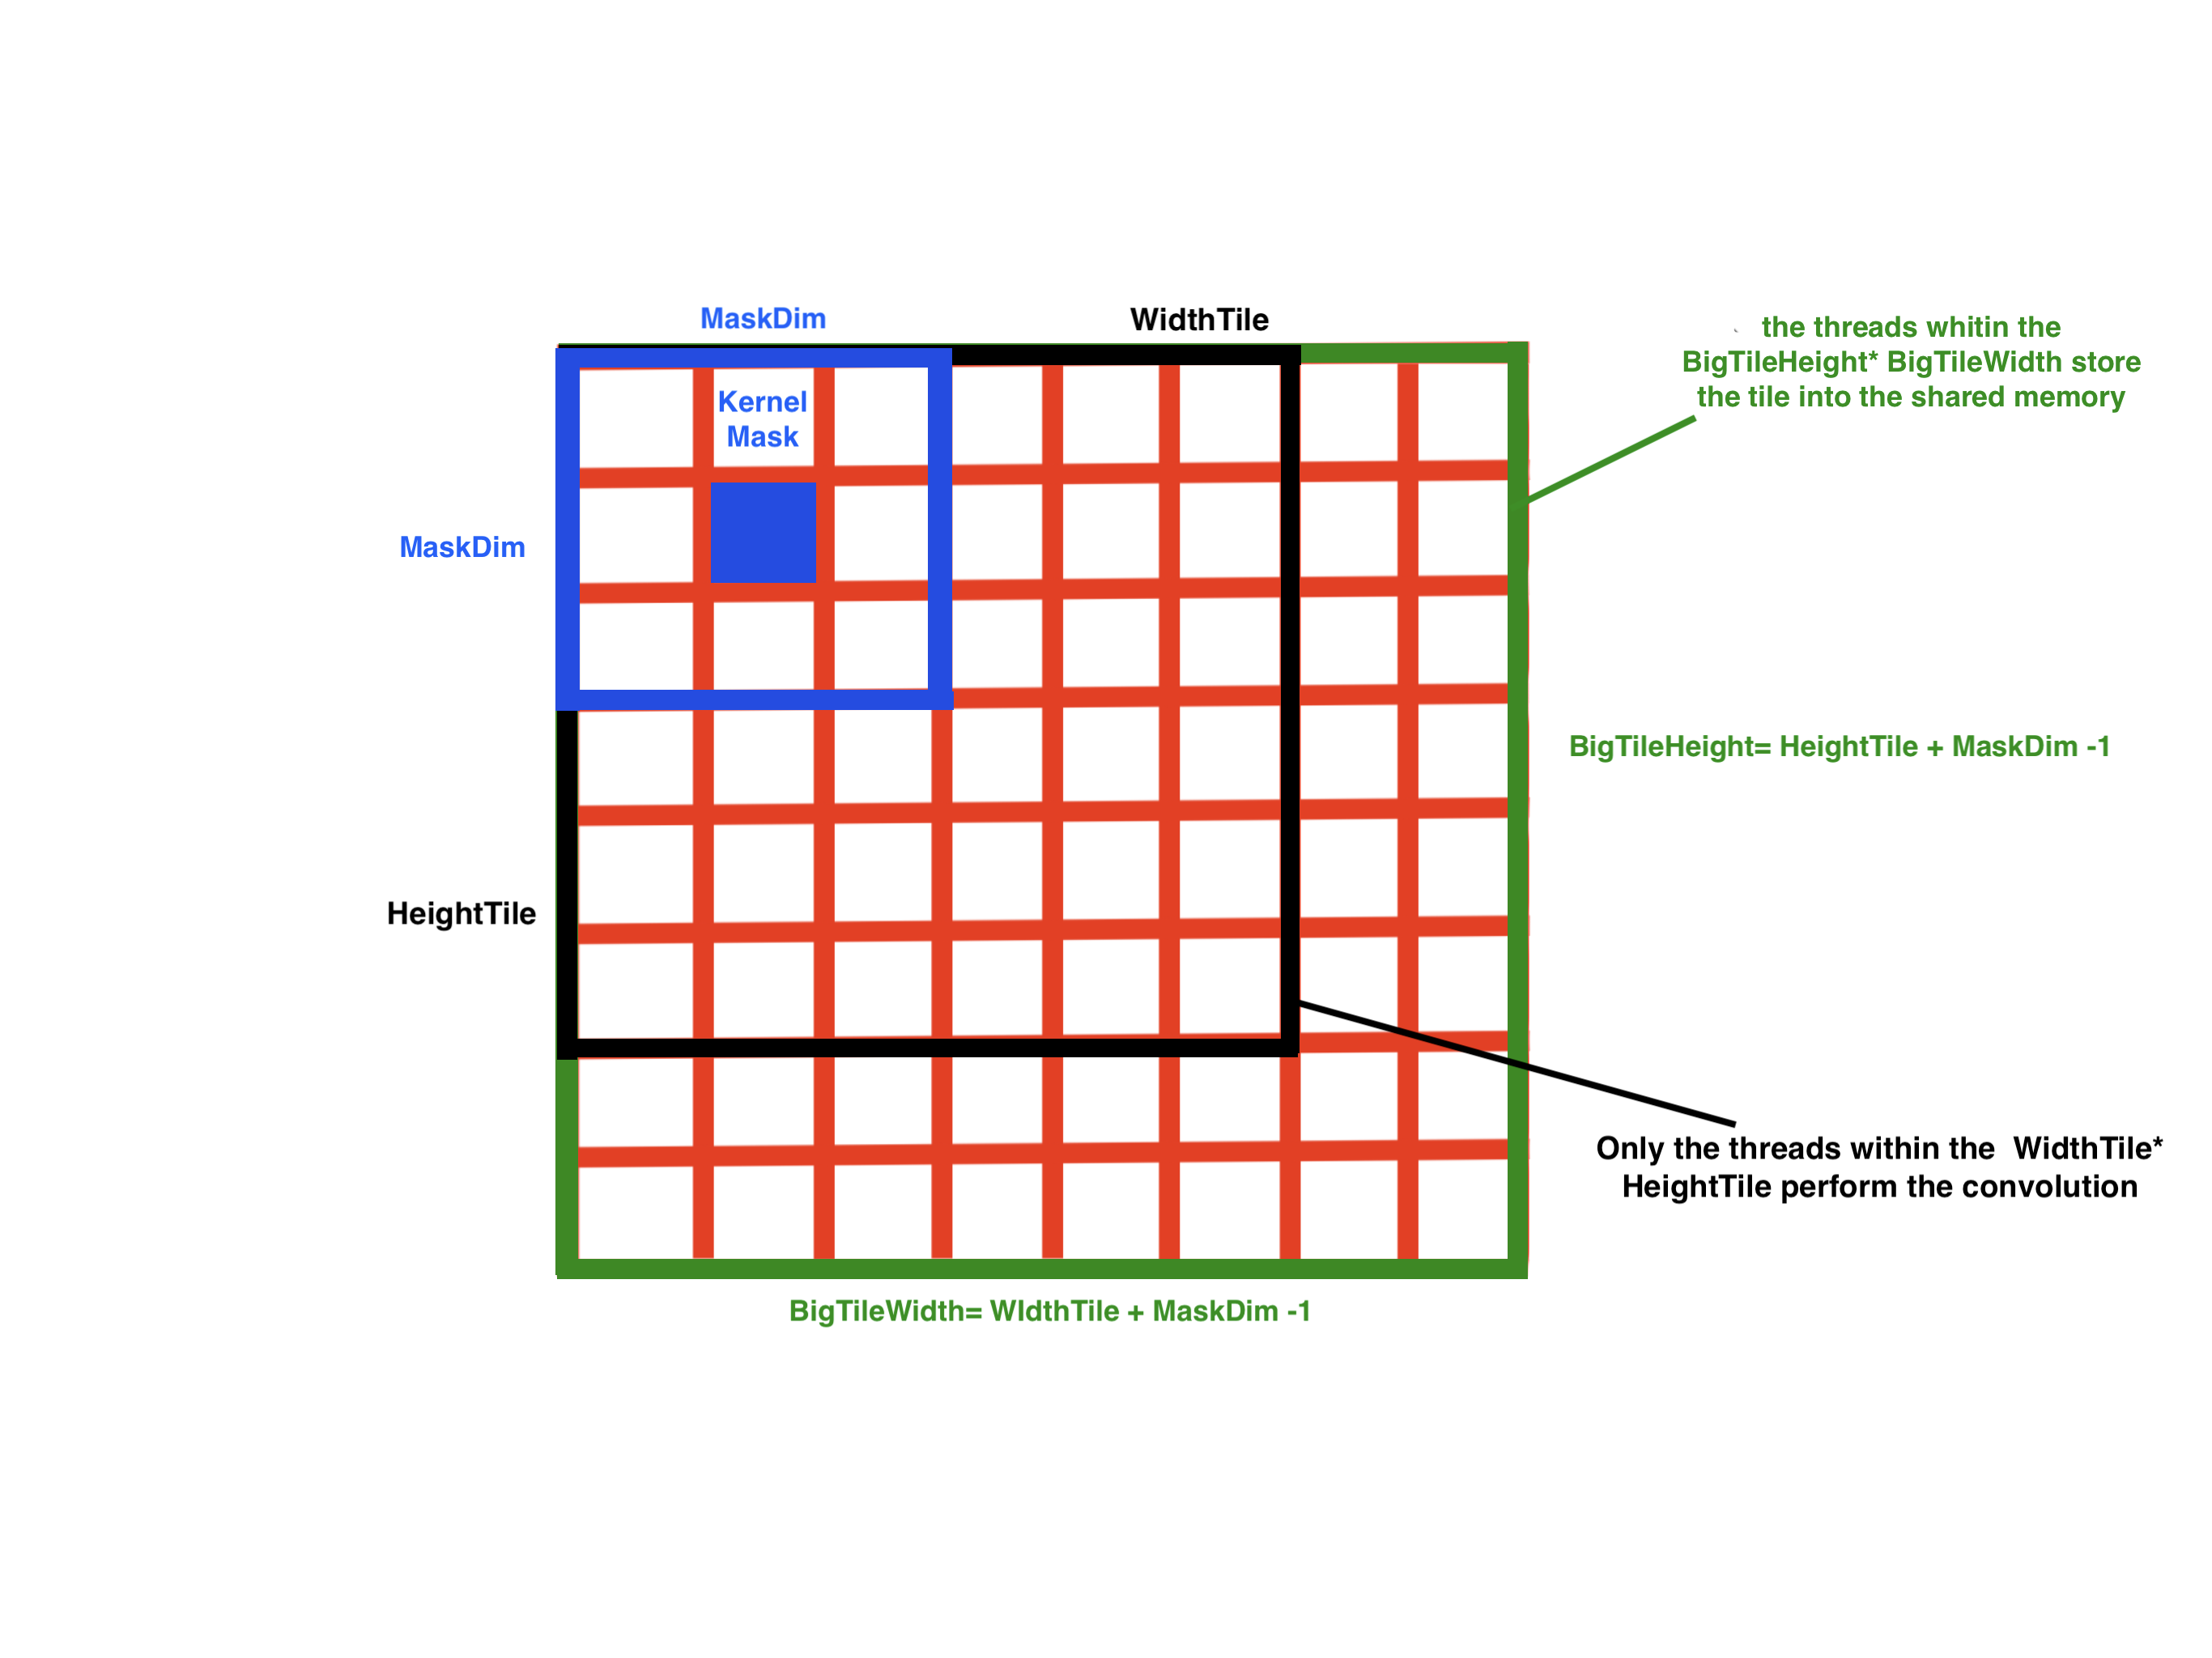
\includegraphics[width=0.5\textwidth]{img/threadsscheme.png}
        \caption{Schematic representation of enhancement process}
        \label{fig:tiling}
    \end{figure}

    \subsection{Code implementation}
    Taken into account what has been said before, the actual implementation has a more direct way of performing the cut, enlargement and convolution.
    The initial version of the algorithm did cut, enlargement and convolution in three different CUDA call, but this was not the most efficient way of doing it.\\
    The final version, instead, performs the whole process in a single CUDA call, which is called by the main function, and it is the one that is actually executed and demonstrated.
    The program calls \textit{globalCudaUpscaling} if the global memory version is used or \textit{tilingCudaUpscaling} in case the shared memory version is possible.

    \begin{figure}[h]
        \centering
        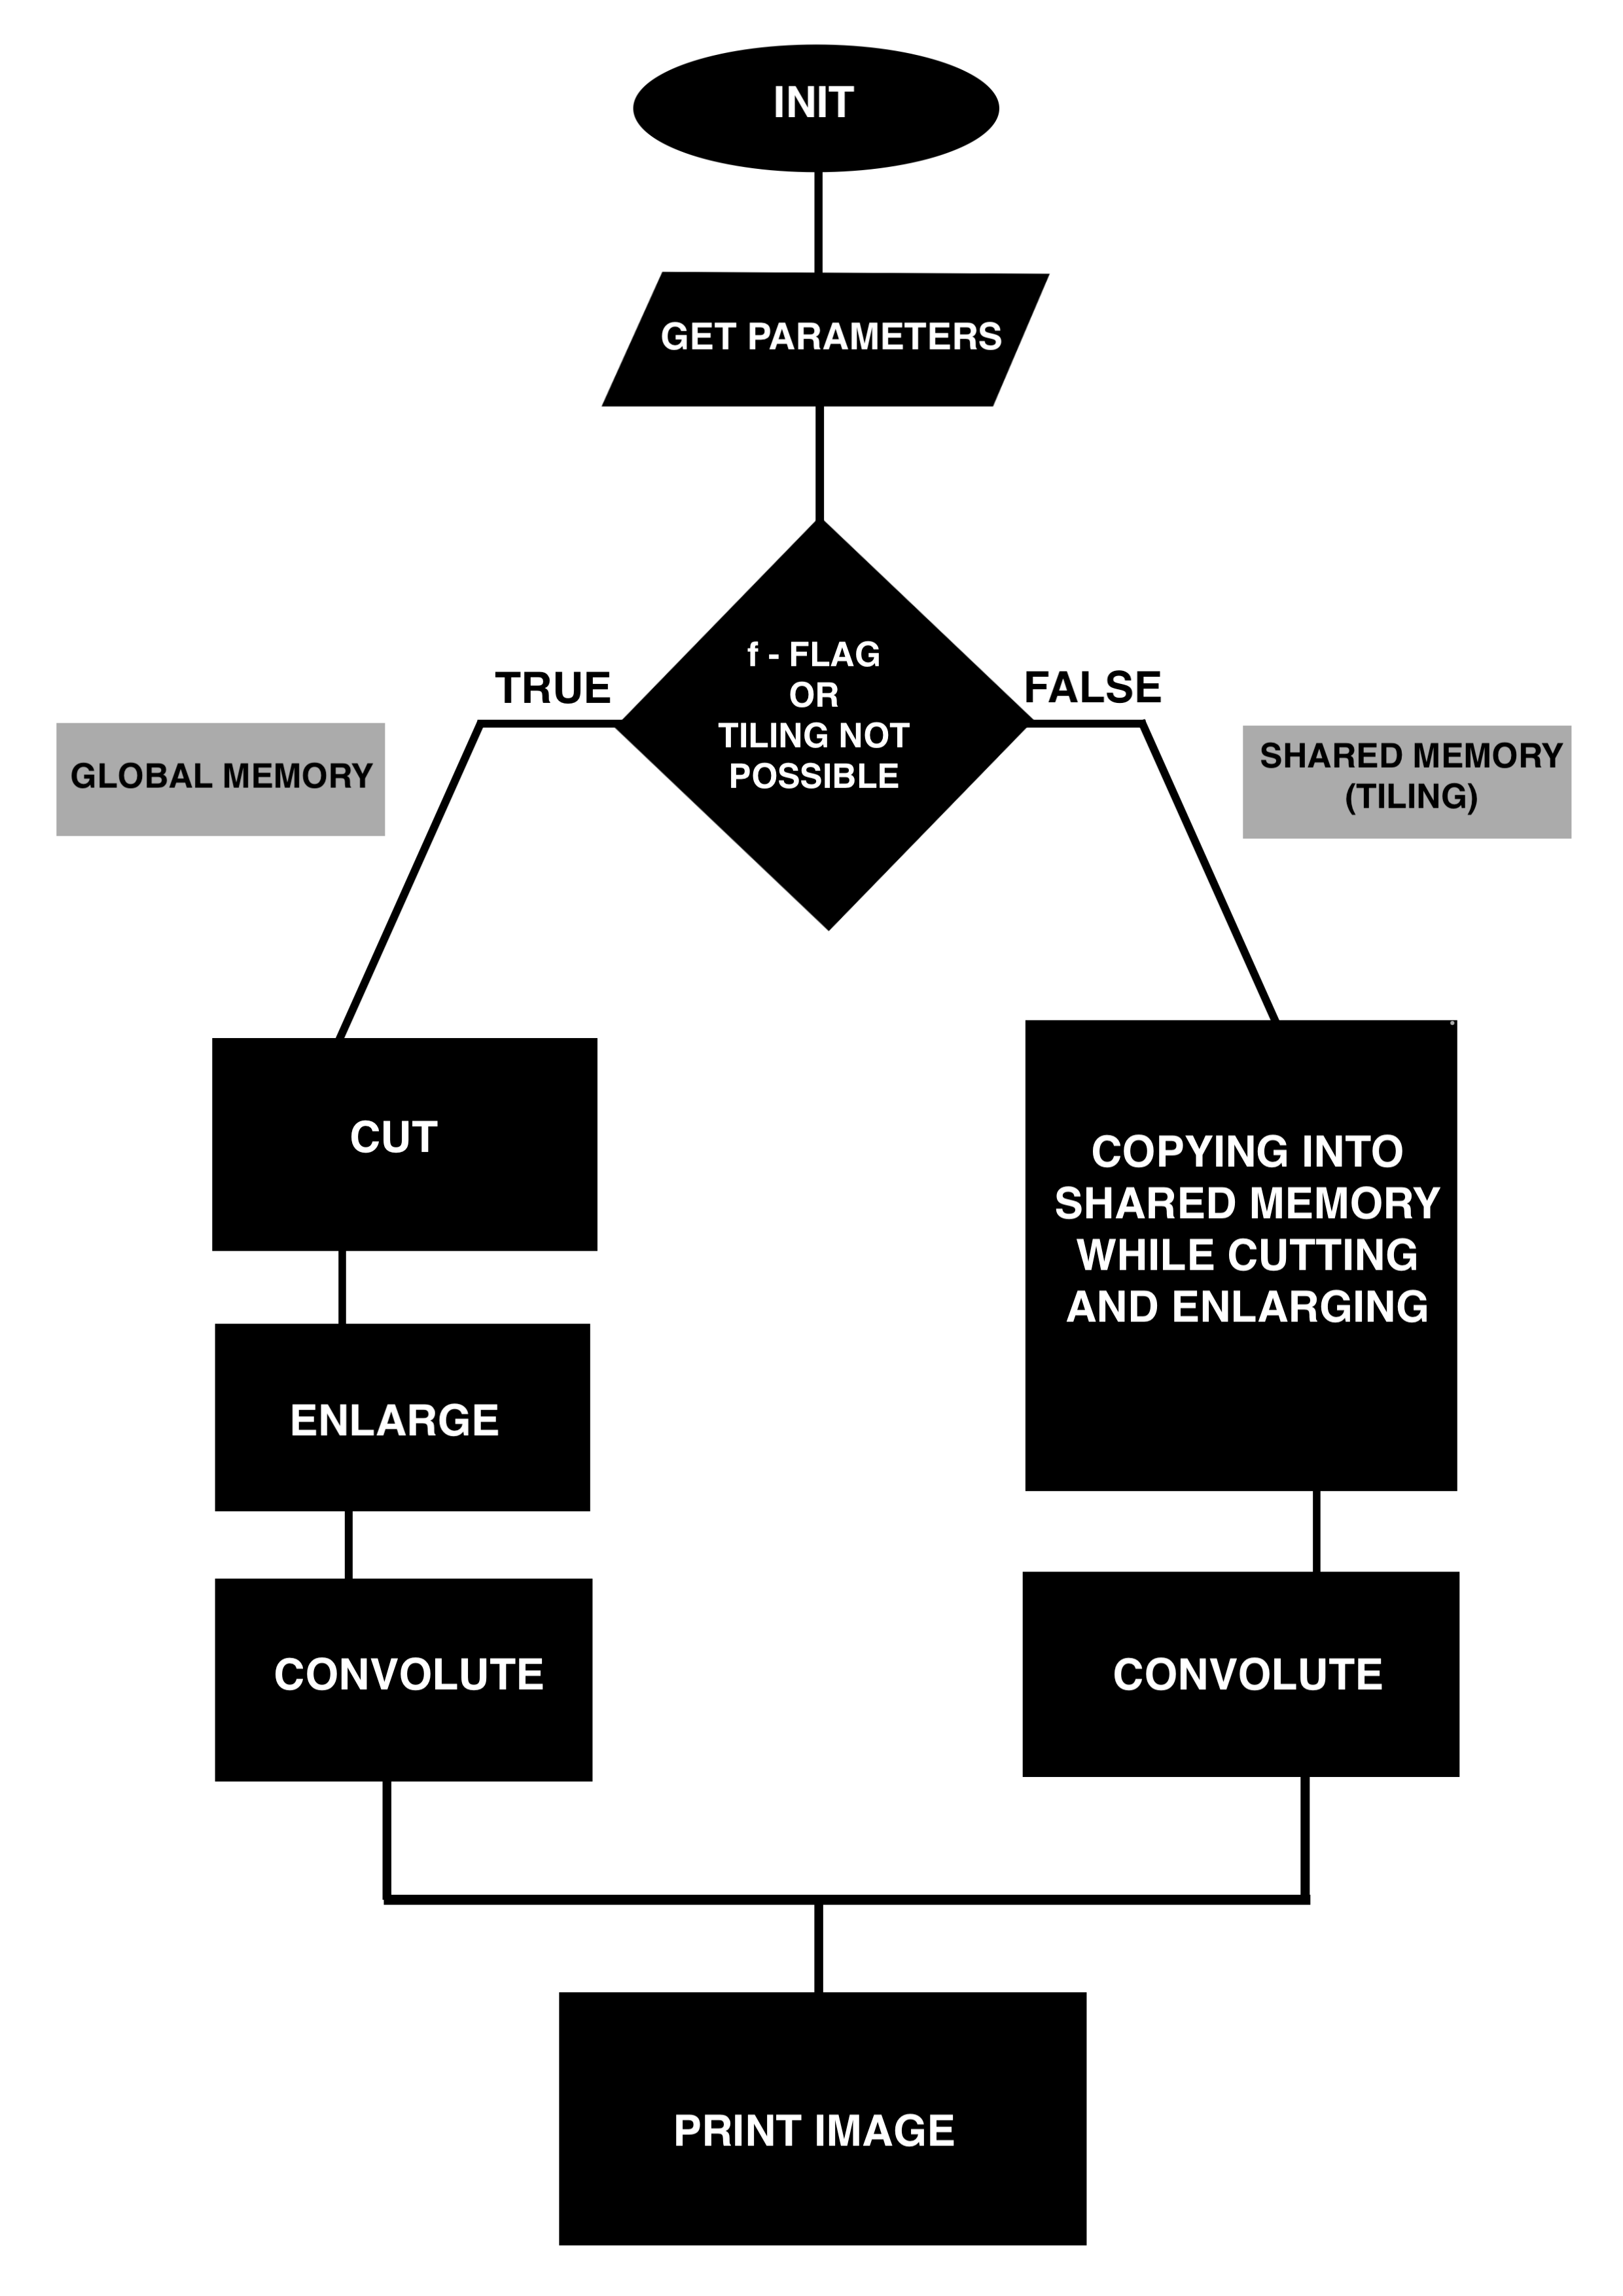
\includegraphics[width=0.7\textwidth]{img/flowchart.png}
        \caption{Flowchart}
        \label{fig:flowchart}
    \end{figure}